
b) Para 40 días antes del vencimiento:

%La tabla ira centrada
\begin{center}
 \renewcommand{\arraystretch}{1.5}% Margenes de las celdas
 %Creación de la cuadricula de 3 columnas
 \begin{longtable}[H]{|p{0.33\linewidth}|p{0.33\linewidth}|p{0.33\linewidth}|}
 	%Creamos una linea horizontal
 	\hline
 	%Definimos el color de la primera fila
 	\rowcolor[HTML]{FFB183}
 	%%%%% INICIO ASIGNACIÓN FECHA FOCAL %%%%%%%
 	%%%%%%%%%% INICIO TITULO
 	%Lo que se hace aquí es mezclar las 3 columnas en una sola
 	\multicolumn{3}{|c|}{\cellcolor[HTML]{FFB183}\textbf{1. Asignación período focal}}                   \\ \hline
 	%%%%%%%%%% FIN TITULO
 	%%%%% INICIO DECLARACIÓN DE VARIABLES %%%%%%%
 	\multicolumn{3}{|c|}{$pf : \frac{40}{365} \ = \ 0.1096 \textit{ pav}$}                                       \\ \hline
 	%%%%%%%%%% INICIO TITULO
 	%Lo que se hace aquí es mezclar las 3 columnas en una sola
 	\multicolumn{3}{|c|}{\cellcolor[HTML]{FFB183}\textbf{2. Declaración de variables}}                 \\ \hline
 	%%%%%%%%%% FIN TITULO
 	%%%%%%%%%% INICIO SUBTITULO
 	\multicolumn{1}{|c|}{\cellcolor[HTML]{FFB183}\textbf{Valores monetarios}}    & 
 	\multicolumn{1}{|c|}{\cellcolor[HTML]{FFB183}\textbf{Valores no monetarios}} &
 	\multicolumn{1}{|c|}{\cellcolor[HTML]{FFB183}\textbf{Incógnitas}}  \\ \hline
 	%%%%%%%%%% FIN SUBTITULO
 	%%%%%%%%%% INICIO DE MATEMÁTICAS
 	%Cada & hace referencia al paso de la siguiente columna
 	$F =  5{.}000{.}000\ COP$  & 	$i  = 30\%\textit{pav}$                         & $P_{v} = \ ? \textit{ COP} \% $  \\
 	&$n = \frac{40}{365} = 0.1096\ pav  $   &  $V_{v} =\ ?\ COP  $\\
 	 &$Comision = 0.5\% \textit{pav}$ & \\                          
 	
 	%%%%%%%%%% FIN DE MATEMÁTICAS
 	%%%%% FIN DECLARACIÓN DE VARIABLES
 	
 	
 	%%%%% INICIO FLUJO DE CAJA
 	\rowcolor[HTML]{FFB183}
 	\multicolumn{3}{|c|}{\cellcolor[HTML]{FFB183}\textbf{3. Diagrama de flujo de caja}}                \\ \hline
 	\multicolumn{3}{|c|}{ 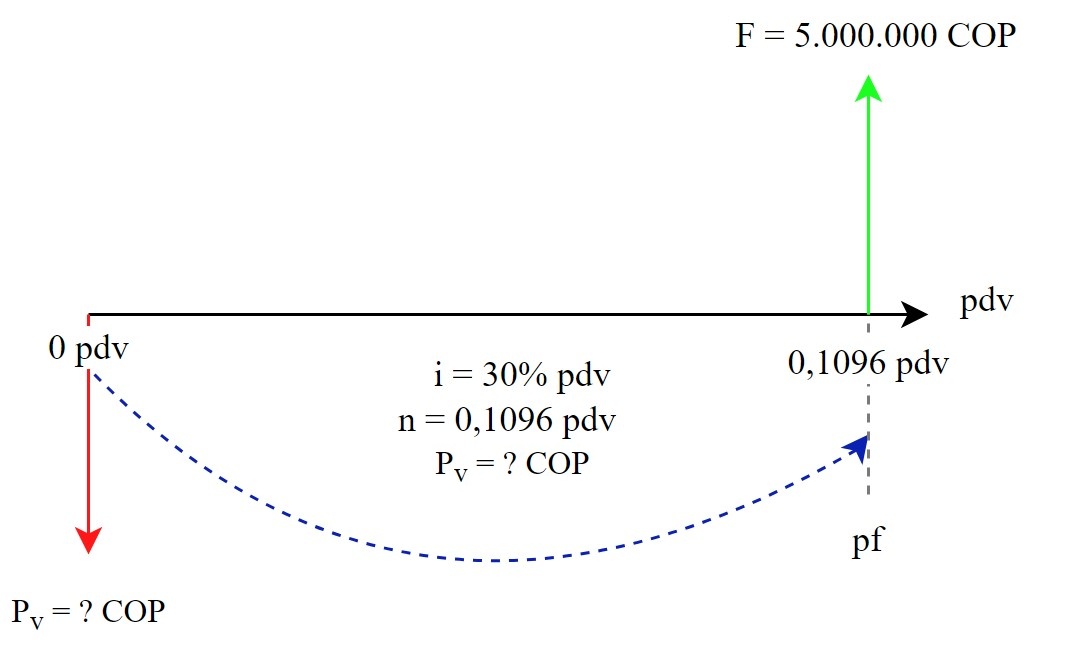
\includegraphics[trim=-5 -5 -5 -5 , scale=0.55, width=16.4 cm, height = 10.5 cm]{3_Capitulo/img/ejemplos/7/7.1.b.png} }  \\ \hline
 	
 	%%%%%% FIN FLUJO DE CAJA

    \rowcolor[HTML]{FFB183}
		\multicolumn{3}{|c|}{\cellcolor[HTML]{FFB183}\textbf{4. Declaración de fórmulas}} \\ \hline
		\multicolumn{3}{|c|}{$F = P(1 + i)^n$ \hspace{2mm} Valor futuro} \\ \hline
    
 	\rowcolor[HTML]{FFB183}
 	\multicolumn{3}{|c|}{\cellcolor[HTML]{FFB183}\textbf{5. Desarrollo matemático}}                    \\ \hline
 	%Mezclamos 3 columnas y pondremos el dibujo
 	%%%%%%%%%%%%% INSERCIÓN DE LA IMAGEN
 	%Deberán descargar las imágenes respectivas del drive y pegarlas en la carpeta
 	%n_capitulo/img/ejemplos/1/capitulo1ejemplo1.pdf  (el /1/ es el numero del ejemplo)
 	\multicolumn{3}{|C{\linewidth}|}{
 		\vspace{4mm}
 		Para el mercado extrabursátil (fuera de bolsa)
 		\vspace{1mm}
 		$V_{veb} = (5{.}000{.}000 \ COP) (1 + 0,3)^\frac{-40}{365} =  4{.}858{.}285,82\  COP $
 		
 		$P_{veb} = \frac{4{.}858{.}285,29}{5{.}000{.}000} = 0,9716 $ 
 	}                                                                                                   \\ \hline
 	
 	%%%%% INICIO DECLARACIÓN FORMULAS
 	%%%%%%%%%%% INICIO TITULO
 	\rowcolor[HTML]{FFB183}
 	
 	%%%%%% INICIO RESPUESTA
 	\rowcolor[HTML]{FFB183}
 	%%%%%%%%%%INICIO TITULO
 	\multicolumn{3}{|c|}{\cellcolor[HTML]{FFB183}\textbf{6. Respuesta}}                                \\ \hline
 	%%%%%%%%%% FIN TITULO
 	%%%%%%%%%% INICIO RESPUESTA MATEMÁTICA
 	\multicolumn{3}{|C{\textwidth}|}{\newline
 		$V_{veb} =  4{.}858{.}285,82\ COP$
        
 		$P_{veb} = 97,16 \textit{ COP}\%$
 	}                                                                                                  \\ \hline
 	%%%%%%%%%% FIN MATEMÁTICAS
 	%%%%%% FIN RESPUESTA"
 	
 \end{longtable}
 %Se crean dos lineas en blanco para que no quede el siguiente texto tan pegado
 %\newline \newline %USARLO SI CREES QUE ES NECESARIO
 
\end{center}
